\documentclass{scrbook}
\usepackage{amsfonts}
\usepackage{amsmath}
\usepackage{float}
\usepackage{geometry}
\usepackage{graphicx}
 \geometry{
 a4paper,
 total={170mm,257mm},
 left=20mm,
 top=20mm,
 }
\begin{document}
\author{Martin Linhard}
\title{Gerätelehre - Zusammenfassung}
\maketitle
\newpage
\tableofcontents
\KOMAoptions{open=any}
\chapter{Inhalt von Notfallrucksack/Sauerstofftasche/Schienentasche}
\section{Notfallrucksack}
Der Rucksack besteht aus einem großen "Hauptraum" sowie 2 Taschen an der Vorderseite.
Im Hauptraum sind an den beiden Seiten jeweils Taschen mit Klettverschluss befestigt.
\subsection*{Seite A}
\begin{figure}[H]
    \centering
    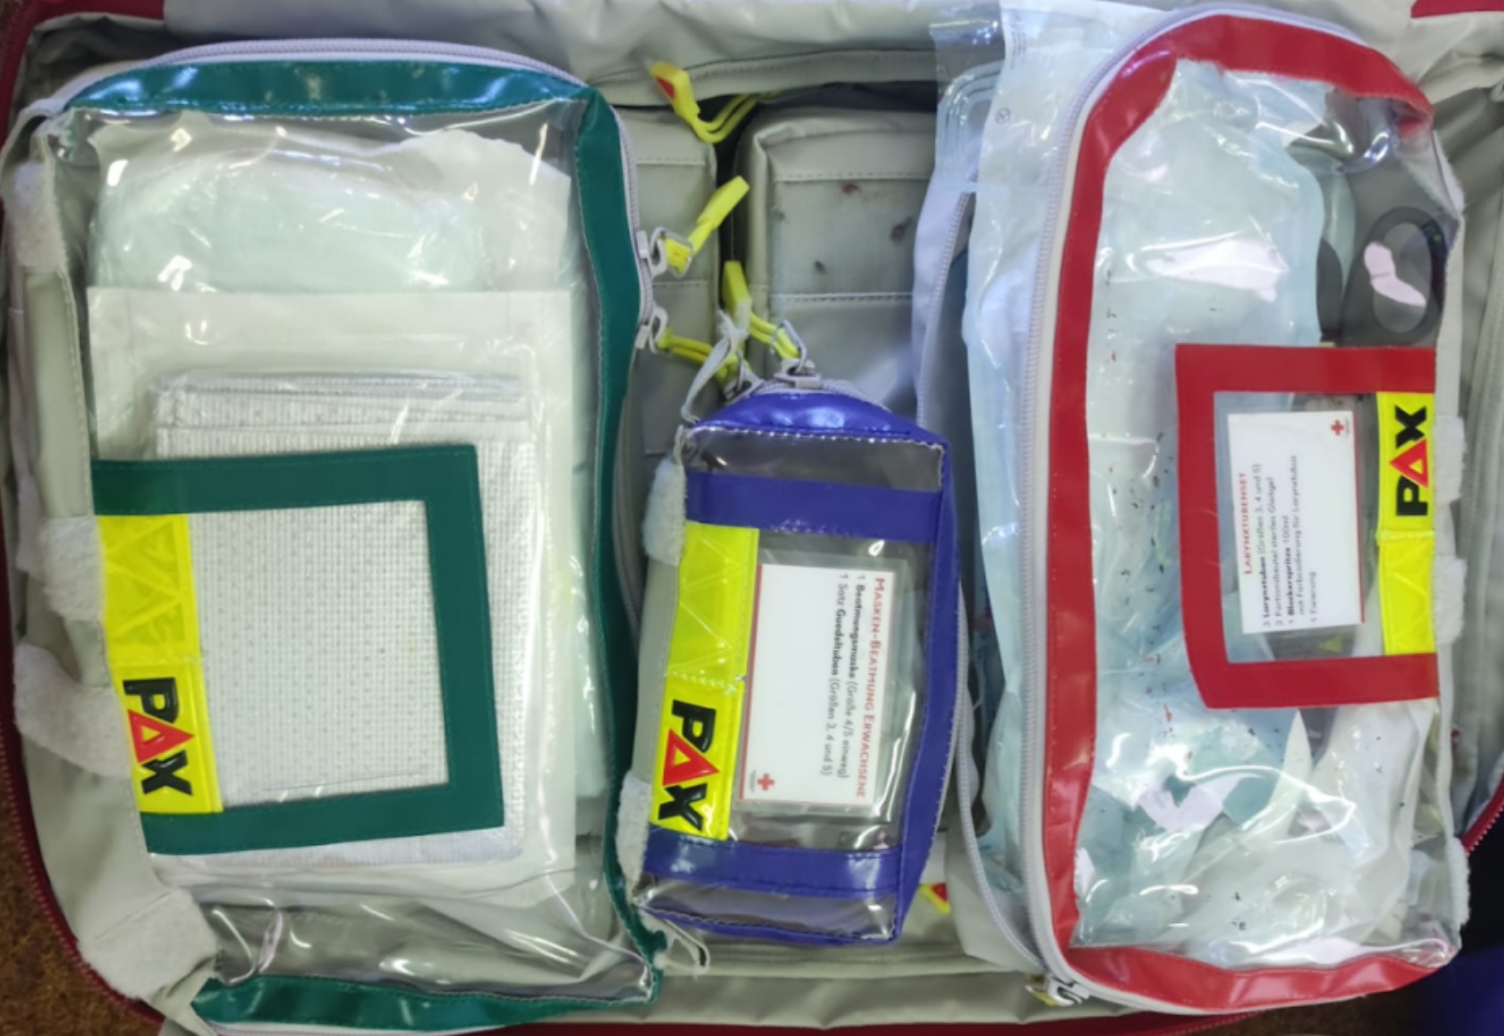
\includegraphics[width=\textwidth]{res/rucksack_a.png}
\end{figure}
\begin{itemize}
    \item Rote Tasche: Larynx Tubus (in 3 Größen) inkl. Zubehör (Blockerspritze, Gleitgel, Etwas zum Fixieren)
    \item (Kleine) blaue Tasche: Guedel Tubus (in 3 Größen)
    \item Grüne Tasche: Wundauflagen (saugende/metallische) \& Verbandmaterial
\end{itemize}
\subsection*{Seite B}
\begin{figure}[H]
    \centering
    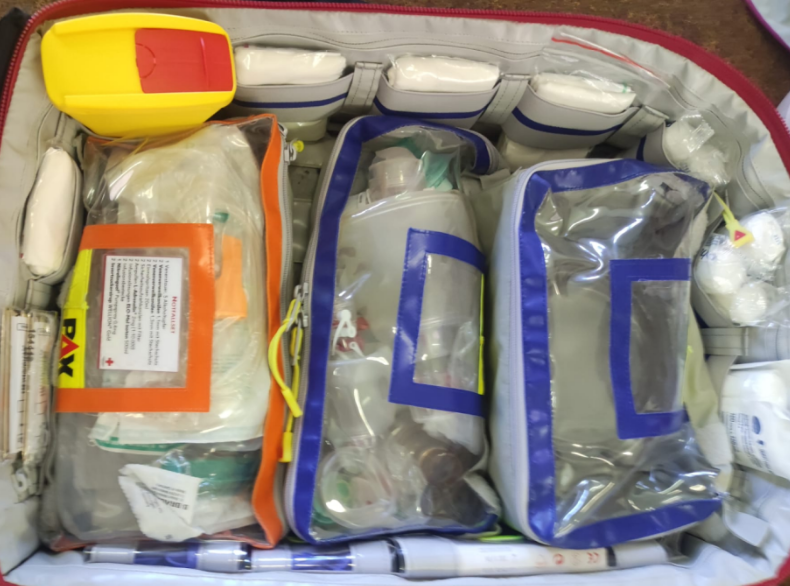
\includegraphics[width=\textwidth]{res/rucksack_b.png}
\end{figure}
\begin{itemize}
    \item Blaue Taschen: Beatmungsbeutel inkl. Zubehör (Luftfilter\dots)
    \begin{itemize}
        \item Je eine Tasche für Erwachsene und Kinder + Säuglinge
    \end{itemize}
    \item Orange Tasche: Material für venösen Zugang / Infusionen
    \item Am Rand: Contamed-Box (Stichfester Behälter für Nadeln etc.), Mullbinden, Wärmedecken, Dreickstücher, Handschuhe
\end{itemize}

\subsection*{Vorderseite Oben - Diagnostik}
\begin{figure}[H]
    \centering
    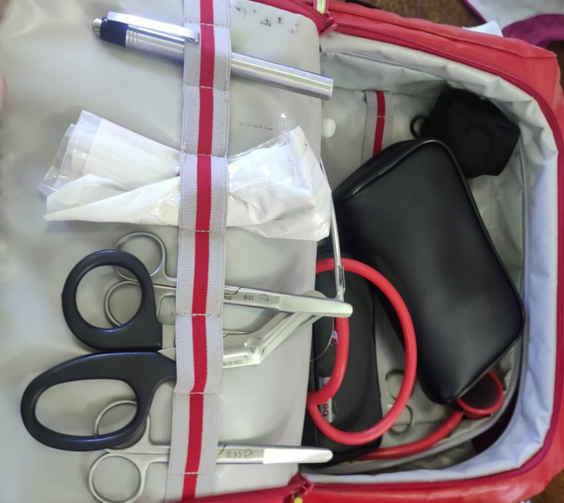
\includegraphics[scale=.5]{res/rucksack_vorne_oben.png}
\end{figure}
\begin{itemize}
   \item Pupillenlampe
   \item Eigentumsbeutel
   \item Scheren
   \item Stethoskop
   \item Pulsoximeter 
   \item Blutzuckermessgerät
   \item Defibrillator 
\end{itemize}

\subsection*{Vorderseite Unten}
\begin{figure}[H]
    \centering
    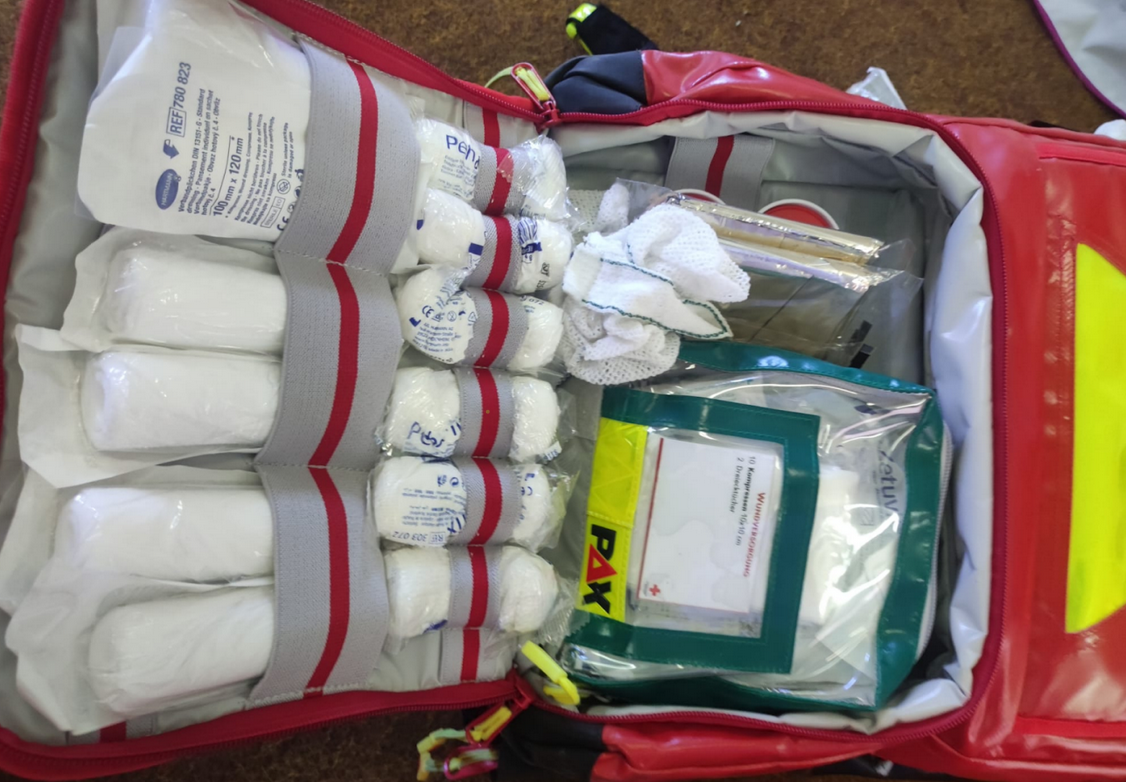
\includegraphics[scale=.5]{res/rucksack_vorne_unten.png}
\end{figure}
\begin{itemize}
   \item Mullbinden
   \item Kompressen
   \item Momentverband (=Mullbinde mit integrierter Wundauflage)
   \item Dreieckstücher
   \item Wärmedecken
   \item Kopfhaube
   \item Leukoplast 
\end{itemize}

\section{Sauerstofftasche}
\begin{figure}[H]
    \centering
    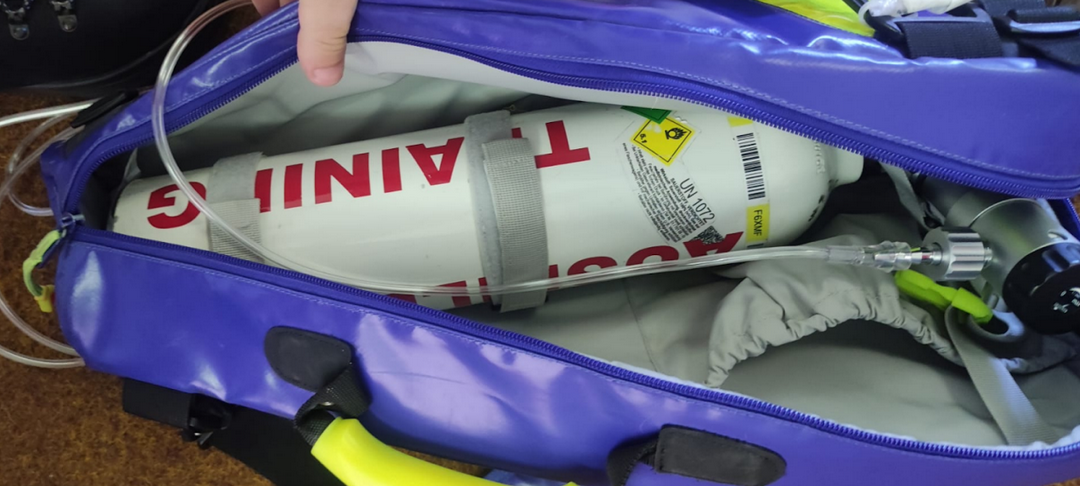
\includegraphics[scale=.5]{res/sauerstofftasche.png}
\end{figure}
\begin{itemize}
    \item Sauerstoffflasche mit Druckminderer
    \item Atemmaske
    \item Nasenbrille
    \item Schlauch
    \item Vor Dienstbeginn kontrollieren, ob genügend Druck vorhanden ist!
\end{itemize}

\section{Schienentasche}
\begin{itemize}
    \item Stiffnecks
    \item Sam Splints (für Unterarm/Knöchel)
    \item Unterschenkel-Vakuum-Schiene
\end{itemize}
\chapter{Umgang mit dem Rettungstuch}
$\implies$ Wichtig: Leintuch verwenden!!
\section{Wegtragen}
\begin{enumerate}
    \item Rettungstuch neben dem Patienten auflegen, unter der einen Hälfte des Patienten positionieren und dann durchziehen
          \begin{enumerate}
              \item Wie bei EH Decke
          \end{enumerate}
    \item Zusammen mit eingewiesener Dritten Person (übernimmt die Füße) die Person wegtragen
\end{enumerate}
\section{Sitzender Transport ("Windeltechnik")}
\begin{enumerate}
    \item Person bitten, aufzustehen
    \item Rettungstuch auf Sessel legen
    \item Person bitten, sich hinzusetzen
    \item Windeltechnik anwenden, wie in Praxis besprochen
    \item Person zu 2. wegtragen
\end{enumerate}
\chapter{Handhabung der Schaufeltrage}
\begin{enumerate}
    \item Trage neben Patienten legen und Größe abmessen (max. 3 Löcher schauen raus) - Beine stehen unten raus, falls zu groß
    \item Trage teilen und auf beiden Seiten in Position bringen
    \begin{enumerate}
        \item Unten: zuerst aufmachen und zuletzt schließen!
    \end{enumerate}
    \item Patienten nacheinander auf beiden Seiten an Schulter und Hüfte anheben, um die Teile unterzuschieben
    \item Teile verbinden
    \item \textbf{Gurte anlegen}
    \item Patient wegtragen
\end{enumerate}
\chapter{Handhabung der Vakuummatratze}
\begin{enumerate}
    \item Matratze auf Trage legen, ausstreifen, sicherstellen, dass Gurte frei sind
    \item Matratze etwas vorabsaugen
    \item Leintuch über Matratze geben, Patienten (z.B. mit Schaufeltrage) auf die Matratze legen
    \item Patient ins Leintuch einwickeln, Luft hineinlassen und Matratze an Patienten anformen
    \item Gurte von der Matratze schließen (Arme wie ein Pharao, Farbcodierungen beachten)
    \item Gurte von der Trage schließen
    \item Luft absaugen (und währenddessen sicherstellen, dass sich die Matratze gut anpasst)
\end{enumerate}
\chapter{Handhabung der Vakuumbeinschiene}
\begin{enumerate}
    \item Fuß unter Spannung setzen
    \item Schiene vorabsaugen und unterlegen (evtl. oberes Ende umklappen)
    \item Schuh ausziehen $\implies$ Achtung: Übergang von Verantwortlichkeit der Spannung auf 2. Sanitäter
    \item Luft hineinlassen, Schiene anformen, Klettverschluss schließen, Gurte schließen
    \item Wechsel von Spannungs-Sanitäter
    \item Absaugen
\end{enumerate}
\chapter{Anlegen der HWS-Schiene beim sitzenden Patienten}
$\implies$ Ein Sanitäter stützt während dem ganzen Vorgang die HWS!
\begin{enumerate}
    \item Kleidung entfernen
    \item HWS richtig einstellen $\implies$ Handkante\dots
    \item Stiffneck unter das Kinn drücken und dann um den Kopf biegen; Klettverschlüsse fixieren
\end{enumerate}
\chapter{Umgang mit der Krankentrage und dem Fahrgestell, Demonstration der Funktionen}S
\begin{itemize}
    \item Roter Hebel $\implies$ Höhe stufenweise anpassen
    \item Trage vom Fahrgestell entkoppeln ($\implies$ Grüner Knopf; außerdem um Trage in RTW zu schieben)
    \item Lenksperre für die vorderen Räder (nur bei Stryker)
    \item Unterkörper/Oberkörper hochlagern, Knierolle simulieren
    \item Infusionsständer
    \item Bremsen
    \item Halme
\end{itemize}
\chapter{Umgang mit dem Tragsessel}
\begin{itemize}
    \item Tragestangen ein/aus fahren
    \item Seitenteile abmontieren, um z.B. Personen vom Sessel zu verlagern
    \item Fußablage (Achtung: Verletzungsgefahr, wenn Patient durch Öffnung durchrutscht!)
\end{itemize}
\chapter{Sauerstoffinhalation mit Maske und Reservoir, Wechsel der Sauerstoffflasche}
\section{Inhalation mit Maske und Reservoir}
\begin{itemize}
    \item Reservoir muss gefüllt sein, bevor Maske aufgesetzt wird
    \item Bei Rettung aus vergifteter Atmosphäre / Tauchunfall wird in den meisten Fällen die CPAP Maske verwendet, sofern sie der Patient toleriert
\end{itemize}
\begin{figure}[H]
    \centering
    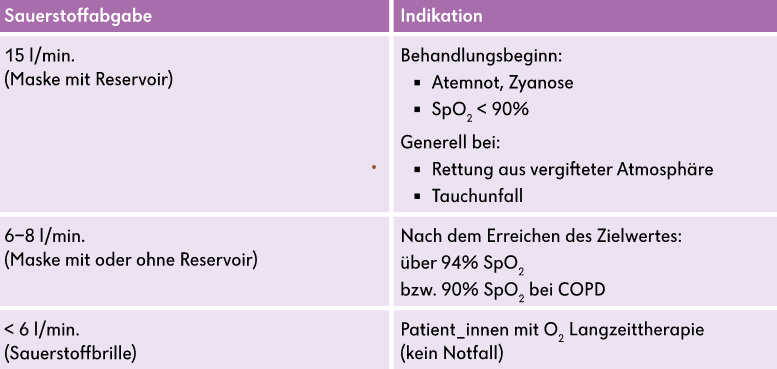
\includegraphics[width=\textwidth]{res/sauerstoff.png}
\end{figure}
\section{Wechsel der Sauerstoffflasche}
\begin{enumerate}
    \item Im Lager muss vermkert werden, welche Flaschen entnommen werden
    \item Bei der neuen Flasche soll (bevor der Druckminderer aufgesetzt wird) 1x kurz aufgedreht werden, damit Staub entfernt wird
    \item Danach kontrollieren, ob Flasche den erwüschten Druck enthält
\end{enumerate}
\chapter{Anwendung der Pulsoxymetrie}
\begin{itemize}
    \item Das Gerät wird eingeschaltet und auf einen Finger geclipt
    \item Zeigt dann Puls und Sauerstoffsättigung an
    \item Messungenauigkeiten können z.B. durch Nagellack, Handcreme, schlechter Durchblutung der Finger entstehen
          \begin{itemize}
              \item Nagellack $\implies$ Gerät kann auch seitlich angebracht werden
          \end{itemize}
\end{itemize}
\section*{Pulswerte}
\begin{figure}[H]
    \centering
    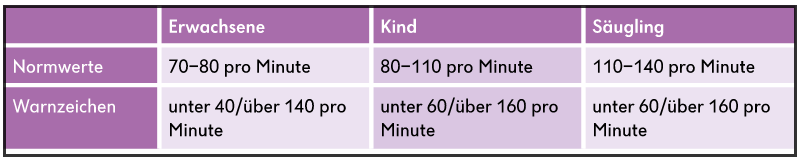
\includegraphics[width=\textwidth]{res/puls.png}
\end{figure}
\chapter{Handhabung des elektrischen Absaugers, Absaugen der Mundhöhle}
\begin{itemize}
    \item 3 Kathetergrößen: Orange (Erw.), Schwarz (Kinder), Säuglinge (Grün).
    \item Saugleistung überprüfen
          \begin{enumerate}
              \item Einschalten und Ende mit Finger verdecken
              \item Muss 0.8 Bar erreichen (innerhalb von 20 Sekunden)
              \item Wenn ausgeschalten $\implies$ Darf in 10 Sekunden nicht mehr als 0.2 Bar verlieren
          \end{enumerate}
    \item Säuglinge $\implies$ Nur 0.2 Bar verwenden
\end{itemize}
\section*{Absaugen der Mundhöhle}
\begin{enumerate}
    \item Katheter auf Sicht ohne Sog einführen (Fingertip offen)
    \item Das Sekret in kreisenden Bewegungen entfernen
    \item Maximale Einführtiefe $\implies$ Abstand zwischen Mundwinkel und Ohrläppchen
\end{enumerate}
\chapter{Handhabung des Larynxtubus}
\begin{enumerate}
    \item Generell erst ab der Pubertät bzw. für dieses Alter (14 Jahre) üblichen Proportionen einsetzbar
    \item Richtige Tubusgröße bestimmen
          \begin{itemize}
              \item \textbf{Gelb:} $<$ 155 cm
              \item \textbf{Rot:} 155 - 180 cm
              \item \textbf{Violett:} $>$ 180 cm
          \end{itemize}
    \item Tubus entblocken
    \item Tubus mit Gleitgel einschmieren
    \item Kinn mit Chin-Lift heben, Tubus einführen (bis letzte Markierung auf Höhe der Zähne ist)
    \item Spritze mit richtiger Luftmenge füllen und Cuffs blocken
    \item Probebeatmung durchführen
          \begin{itemize}
              \item Erfolgreich: Fixieren
              \item Nicht erfolgreich: Eine Markierung weiter hinaus ziehen, erneut probieren
              \item Noch immer nicht erfolgreich: Andere Tubusgröße ebenfalls 2x testen, sonst Guedeltubus
          \end{itemize}
    \item Fixieren
          \begin{itemize}
              \item Mullbinde halbieren, um den Kopf legen, 2x verknoten, auf die andere Seite des Tubus, Knoten machen $\implies$ Tubus sollte sich zum Ende in einem Mundwinkel befinden
              \item Adapter auf den Tubus stecken und mit Gummi fixieren
          \end{itemize}
\end{enumerate}
\chapter{Handhabung des Beatmungsbeutels für Erwachsene und des Guedeltubus}
\section{Guedeltubus}
\begin{enumerate}
    \item Größe wie beim Katheter abmessen (Mundwinkel - Ohrläppchen)
    \item Tubus um 180° verdreht einsetzen (Chin-Lift) und anschließend umdrehen
\end{enumerate}
\section{Beatmungsbeutel}
\begin{enumerate}
    \item Richtigen Beutel wählen
    \item Richtig zusammenbauen (wenn kein passender Filter vorhanden ist, wird darauf verzichtet!)
    \item Reservoir anfüllen
          \begin{enumerate}
              \item Erwachsene $\implies$ 15l
              \item Kinder $\implies$ 8l
              \item Säuglinge $\implies$ 6l
          \end{enumerate}
    \item Maske auf den Mund aufsetzen; mit C-Griff fixieren
          \begin{itemize}
              \item Erwachsene $\implies$ Unterkiefer hochziehen, um Atemwege freizumachen
              \item Säugling $\implies$ Unterkiefer mit einem Finger in Neutralstellung bringen
              \item Kind $\implies$ Unterkiefer leicht hochziehen, um Atemwege freizumachen
          \end{itemize}
    \item Mit 2 Fingern zusammendrücken
\end{enumerate}
\chapter{Abbindung mit Tourniquet}
\begin{enumerate}
    \item Tourniquet wird eine Handbreit von der Wunde entfernt (Richtung Körper) angelegt und der Gurt festgezogen
    \item Bei den ersten Umdrehungen werden 2 Finger untergeschoben, damit Haut nicht verdreht wird
    \item Danach so lange zudrehen, bis kein Blut mehr austritt
    \item Der Zeitpunkt der Abbindung muss am Gerät (und am besten in anderen Unterlagen) festgehalten werden
    \item Max. 2 Tourniquets verwenden
\end{enumerate}
\chapter{Blutdruckmessung ohne und mit Stethoskop}
\section{Allgemein}
\begin{figure}[H]
    \centering
    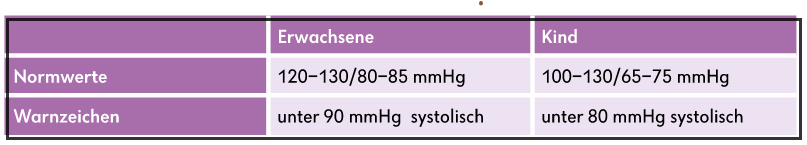
\includegraphics[width=\textwidth]{res/blutdruck.png}
\end{figure}

\section{Ohne Stethoskop - Palpatorisch}
\begin{enumerate}
    \item Manschette um Oberarm legen
    \item Stellschraube schließen, Puls am Arm tasten
    \item So lange aufpumpen, bis kein Puls mehr spürbar ist, dann 2x drücken
    \item Vorsichtig die Stellschraube öffnen, damit Luft langsam entweicht
    \item Sobald Puls wieder spürbar $\implies$ Systolischer Blutdruck
    \item Luft ganz auslassen
\end{enumerate}

\section{Mit Stethoskop - Auskulatorisch}
\begin{enumerate}
    \item Manschette um Oberarm legen
    \item Stellschraube schließen, Puls tasten
    \item So lange aufpumpen, bis kein Puls mehr spürbar ist, dann 2x drücken
    \item Stethoskop in der Ellenbeuge ansetzen
    \item Stellschraube öffnen
    \item Sobald pulsartige Geräusche hörbar sind $\implies$ Systolischer Blutdruck
    \item Geräusche hören auf $\implies$ Diastolischer Blutdruck
    \item Luft ganz auslassen
\end{enumerate}

\chapter{Blutzuckermessung}
\begin{enumerate}
    \item Finger mit Desinfektionsmittel einschmieren und einwirken lassen
    \item Person informieren
    \item Mit Stechhilfe (Entsorgung $\implies$ ContaMed) auf der Seite des Fingers (Ring-/Mittelfinger, nicht dominante Hand)
    \item Ersten Tropfen Blut wegwischen, zweiten Tropfen auf das Messgerät geben
    \item Wunde versorgen
\end{enumerate}
\begin{figure}[H]
    \centering
    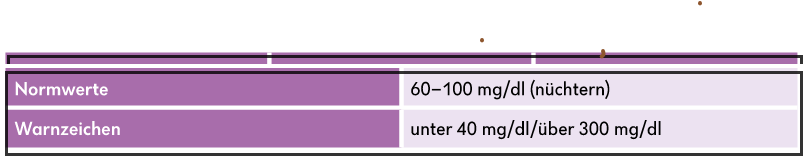
\includegraphics[width=\textwidth]{res/blutzucker.png}
\end{figure}
\end{document}